\documentclass[11pt]{scrartcl}

% Kodierung dieser Datei angeben
\usepackage[utf8]{inputenc}

% Schönere Schriftart laden
\usepackage[T1]{fontenc}
\usepackage{lmodern}
\usepackage {units}
\usepackage{csquotes}

% Tabelle im Querformat
\usepackage{lscape}
\usepackage{pdflscape}

%Pdf einbinden
\usepackage{pdfpages}


% Deutsche Silbentrennung verwenden
\usepackage[ngerman]{babel}

% Bessere Unterstützung für PDF-Features
\usepackage[breaklinks=true]{hyperref}

\KOMAoptions{%
  % Absätze durch Abstände
  parskip=full,%
  % Satzspiegel berechnen lassen
  DIV=calc%
}

% TikZ laden
\usepackage{tikz}

% Verwendete TikZ-Bibliotheken laden
\usetikzlibrary{positioning,automata}
\title{Klasse 5b Festigung des Umfangs einer Fläche}
\author{Felix Liesendahl}
\begin{document}
\maketitle
\tableofcontents
\newpage

\section{Bedingungsanalyse (Beschreibung der Lerngruppe), Einordnung in den Lehrplan, Formulierung der Lernziele}
Die Klasse 5b wurde mir als eine sehr leistungsstarke Klasse beschrieben, die aufgrund von Corona in 2 Gruppen unterteilt ist. Dadurch gibt es in dieser Gruppe 13 Schüler, wobei 9 weiblich und 4 männlich sind.
Da ich die Schüler bereits am Vortag in einer Doppelstunde zur Einführung des Umfangs von Flächen unterrichtete, bin ich bei den Schülern schon bekannt. Davor wurde von der Lehrerin das Thema Flächeninhalt von Flächen abgeschlossen.

In den beiden Stunden zuvor haben die Schüler eine Einführung erhalten was der Umfang ist und kleine Aufgaben erhalten. Da bei manchen Schülern das Verständnis noch nicht gegeben war, wird dies in dieser Stunde nochmals an einem Einfachen Beispiel wiederholt.
Das Thema Umfang gehört zur Geometrie in der 5. und 6. Klasse. Der Umfang wird nach dem Flächeninhalt eingeführt, da die Vorstellung für die Schüler einfacher ist eine Fläche sich vorzustellen als eine Umrandung (vom großem zum kleinem). Im Lehrplan ist für die 5. Klassen vorgesehen ohne Nachkommazahlen zu arbeiten. Dies ist im Buch nicht beachtet worden.

Die Lernziele sind:
SuS können die Formel des Umfangs von Rechtecken ohne Hilfsmittelangeben, an Beispielen anschaulich erläutern und sachgerecht zum Lösen von Problemen anwenden. SuS können den Umfang (und Flächeninhalt) von Quadraten, Rechtecken und aus ihnen zusammengesetzten Figuren messen und berechnen.

\newpage
\section{Tabellarischer Verlauf (Phasen, Fragestellungen, Gelenkstellen, methodisches Vorgehen)}
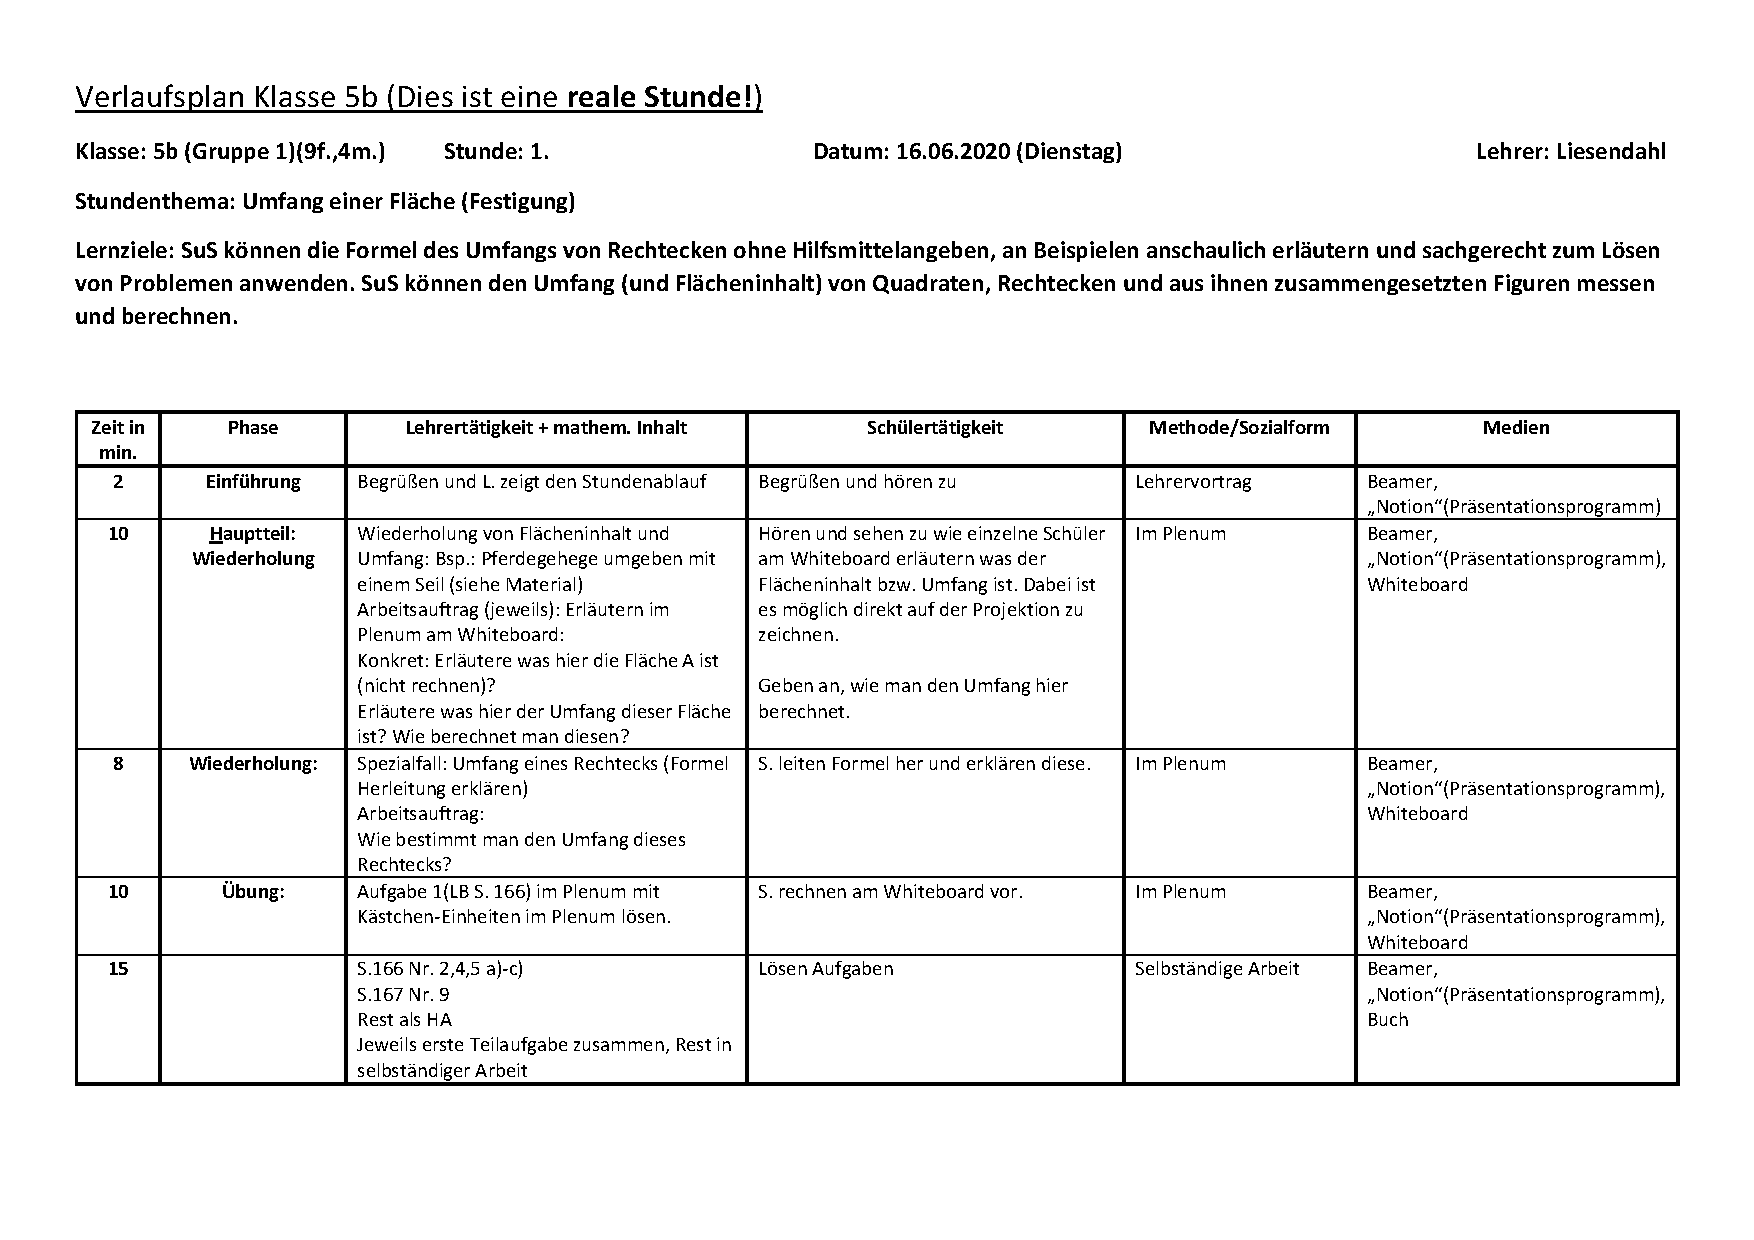
\includepdf[pages=1, landscape] {Verlaufplan_P2}
Gelenkstellen: Zwischen der ersten und zweiten Wiederholung:
\enquote{Da wir nun allgemein den Umfang bestimmt haben, kommen wir jetzt zu einem Spezialfall. Ihr wisst doch noch eine Formel von gestern, für welche geometrische Form war diese und wie lautet sie?} Nach Beantwortung der Form, öffnen der Nächsten Seite (Abbildung mit Rechteck).

Zischen der zweiten Wiederholung zur Übungsphase:
\enquote{Nun besprechen wir die Aufgabe 1 von Seite 166, die ihr gestern angefangen hattet.}

Zwischen erster und zweiter Übungsphase:
\enquote{Schlagt alle das Buch auf Seite 166 auf und löst die hier gezeigten Aufgaben, der Rest wird Hausaufgabe sein.}

\newpage
\section{Beschreibung des tatsächlichen Verlaufs, Erläuterungen zu Abweichungen}
Die Wiederholung hat gut funktioniert und alle Schüler haben den Unterschied zwischen Umfang und Flächeninhalt verstanden. Nicht wie geplant lief dafür die Zeit, da beide Wiederholungen und die Aufgabe 1 auf Seite 166 zusammen 10 min länger dauerten als geplant. Dies kam wahrscheinlich dadurch, dass ich zu viele Schüler am Whiteboard vorrechnen ließ.
Bei der Aufgabe 1 gab es 3 Teilaufgaben, wo es gereicht hätte nur 2 im Plenum vorzurechnen und den Rest mündlich zu besprechen.

Bei der Übungsphase sind die Schüler nur bis Aufgabe Nr. 4 gekommen und hatten daher mehr als Hausaufgabe auf.

\newpage
\section{Reflexion der Lernziele, Reflexion der gewählten Methoden und Schlussfolgerungen für die eigene Arbeit. Gehen Sie hier besonders darauf ein, was Sie anders gemacht hätten, wenn Sie die ganze Klasse unter \enquote{Normalbedingungen} unterrichtet hätten!}
SuS können die Formel des Umfangs von Rechtecken ohne Hilfsmittelangeben, an Beispielen anschaulich erläutern und sachgerecht zum Lösen von Problemen anwenden. SuS können den Umfang (und Flächeninhalt) von Quadraten, Rechtecken und aus ihnen zusammengesetzten Figuren messen und berechnen.
Die hier genannten Lernziele konnte ich beim herumgehen während der selbständigen Arbeit als auch vorher bei der Besprechung gut nachvollziehen.
Besonders ließ sich ein Unterschied zum Vortag ausmachen. D.h. vorher haben viele die allgemeine Formel des Umfangs mit der des Rechtecks verwechselt oder gemixt. Vielen war noch nicht klar, wie bei Aufgabe 1 Kästchen abgezählt werden müssen, um den Umfang zu bestimmen.

Methodisch gesehen war die Wahl der Wiederholung im Plenum sehr gut für das Alter der Schüler. Am Vortag hatte ich versucht mit mehr eigenständige Arbeit vorzugehen, aber dies bringt eher Unruhe und die Schüler arbeiten nicht gleich schnell noch effizient.

Diese Methode werde ich auch in Zukunft für diese Klassenstufe anwenden, da die Schüler viel angeleitet werden müssen.

Unter \enquote{Normalbedingungen} wäre die Klasse aus 26 Schülern. D.h. hier hätte man die momentan nicht erlaubte Gruppenarbeit verwenden können. Die Aufgabe Nr. 2 auf Seite 166 ist eigentlich für die Partnerarbeit ausgelegt. Die Schüler hätten Aufgabenteile untereinander vergleichen können und bei Unklarheiten bzw. Lösungen zusammen im Plenum vorstellen können.
Von zu viel Gruppenarbeit ist, dann aber trotzdem abzusehen, da sonst zu viel Unruhe reinkommt und somit die Schüler sich gegenseitig ablenken.
Es sollte ein angemessenes Maß an Methodenvielfalt angewendet werden.

\newpage
\section{Material}
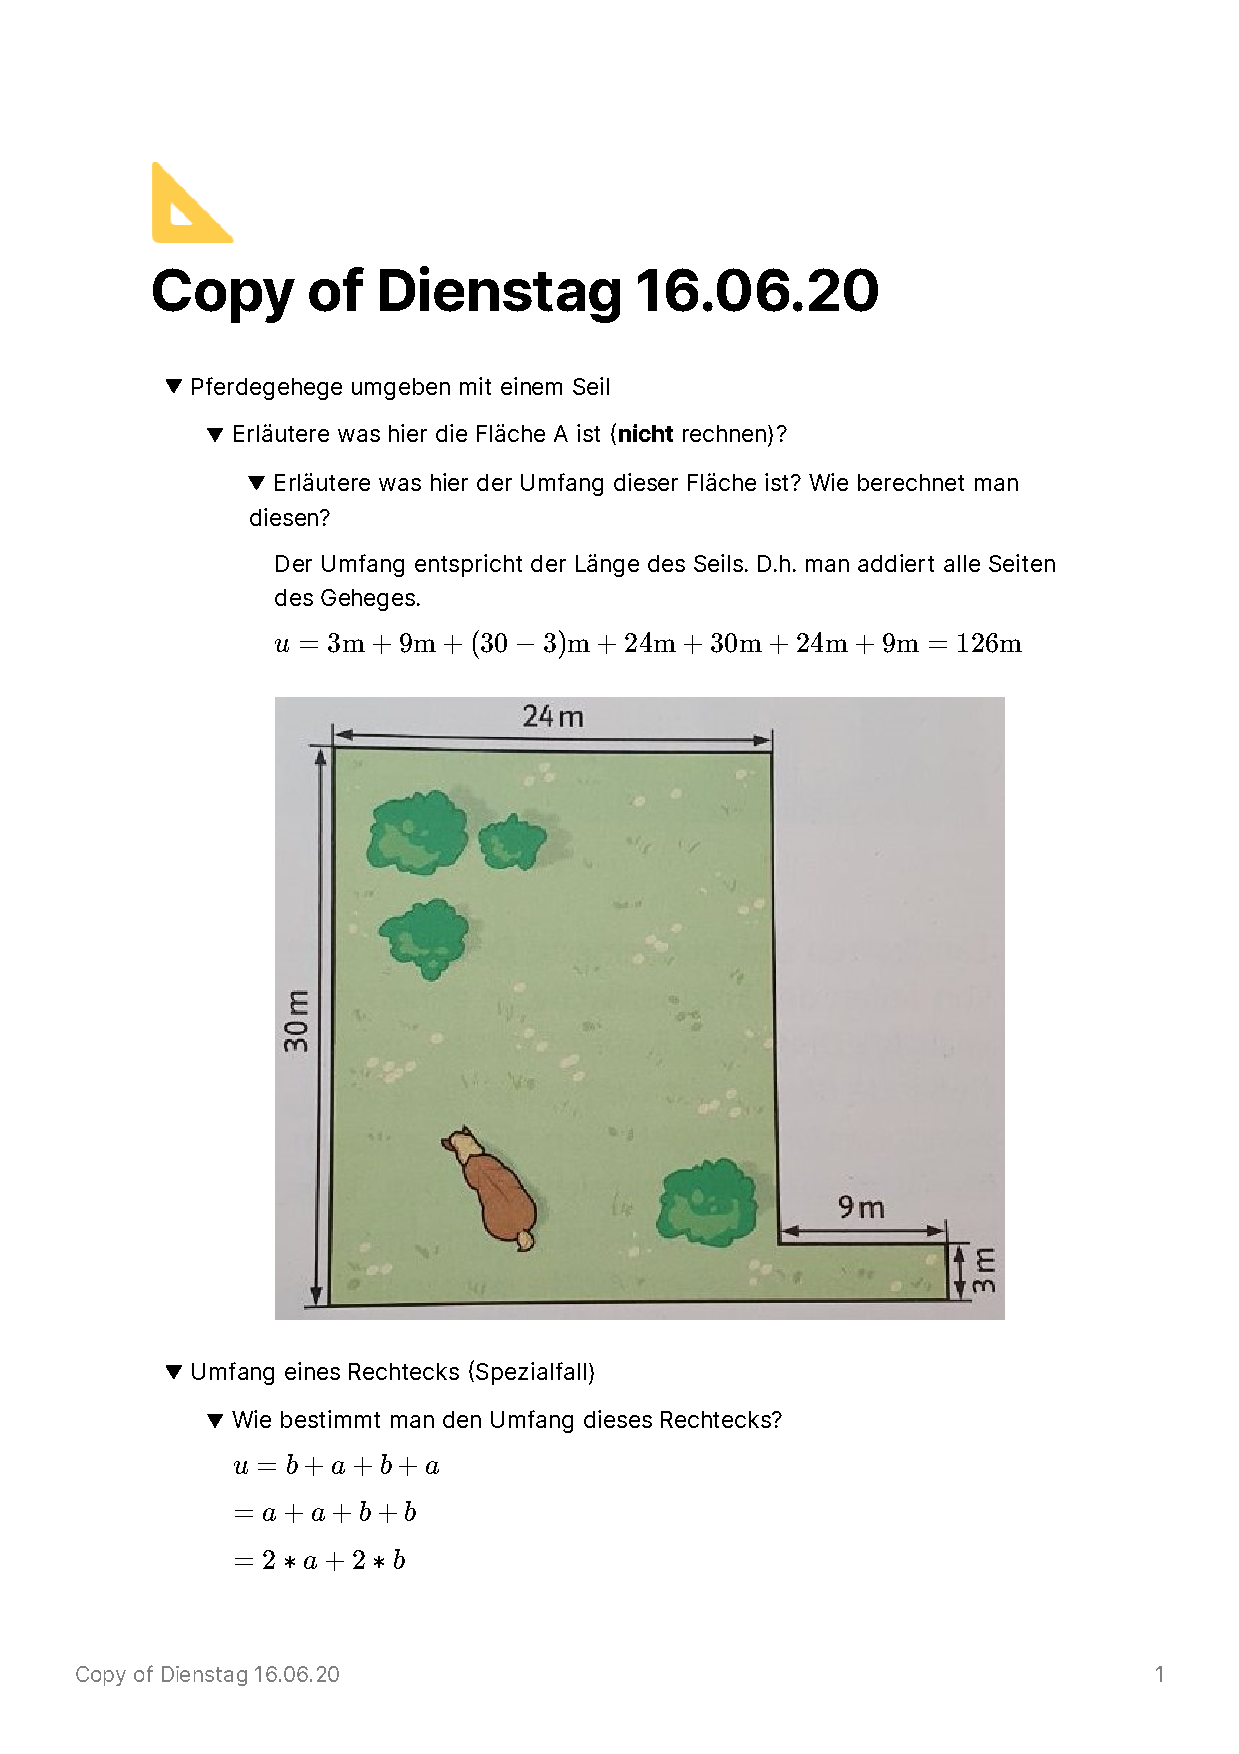
\includepdf[pages=1] {Umfang_Klasse_5_16.06.20}
\includepdf[pages=2] {Umfang_Klasse_5_16.06.20}
\includepdf[pages=3] {Umfang_Klasse_5_16.06.20}






\end{document}
